\chapter{Introduction Generale}

\section{Contexte et Problematique}

Le systeme juridique marocain repose sur un ensemble riche et complexe de textes de loi couvrant de multiples domaines : droit penal, code de la route, droit de la famille, droit civil, droit commercial, procedures judiciaires, droit fiscal, et droit des contraventions. Ces textes, rediges principalement en arabe, sont publies sous forme de documents PDF souvent numerises, ce qui rend leur consultation difficile et chronophage.

Les professionnels du droit --- avocats, magistrats, juristes d'entreprise --- ainsi que les citoyens marocains sont confrontes a plusieurs defis majeurs :

\begin{itemize}
    \item \textbf{Volume et dispersion} : Les textes de loi sont repartis sur des centaines de documents, rendant la recherche d'information longue et fastidieuse.

    \item \textbf{Format non structure} : La majorite des textes historiques existe uniquement au format PDF scanne, rendant la recherche plein-texte impossible sans traitement prealable.

    \item \textbf{Barriere linguistique} : L'arabe juridique utilise un vocabulaire specialise et des formulations complexes, creant un fosse entre la langue du citoyen et celle du legislateur. Les solutions de recherche existantes reposent sur des mots-cles exacts, sans capacite semantique.

    \item \textbf{Risque des LLMs generalistes} : Les modeles de langage comme ChatGPT ou Gemini produisent des reponses juridiques plausibles mais non fondees sur les textes de loi marocains. Sans ancrage dans les sources officielles, ces reponses peuvent contenir des inventions d'articles (hallucinations) et induire les utilisateurs en erreur grave.
\end{itemize}

Face a ces defis, une approche innovante s'impose : combiner la puissance des modeles de langage avec un acces direct et verifiable aux sources juridiques marocaines. L'architecture \textbf{RAG (Retrieval-Augmented Generation)} permet precisement cela : chaque reponse generee est ancree dans les textes de loi authentiques prealablement indexes.

\section{Objectifs du Projet}

Ce projet vise a concevoir et implementer un assistant juridique intelligent specialise dans le droit marocain. L'objectif principal est de fournir des reponses juridiques precises et tracables, fondees exclusivement sur les textes de loi authentiques, a travers une interface simple et accessible en langue arabe.

Les objectifs specifiques sont les suivants :

\begin{enumerate}
    \item \textbf{Constitution du corpus} : Construire un pipeline automatise capable d'extraire le texte des documents juridiques marocains (PDF numeriques et numerises), de le nettoyer, de le normaliser, et de le structurer en articles de loi exploitables avec metadonnees.

    \item \textbf{Recherche semantique arabe} : Developper un moteur de recherche hybride (dense + lexical) capable de retrouver les articles de loi pertinents a partir d'une question posee en arabe, avec une tokenisation adaptee a la morphologie de la langue.

    \item \textbf{Generation de reponses fondees et enrichies} : Integrer un modele de langage (LLM) qui genere des reponses juridiques en s'appuyant exclusivement sur les textes de loi recuperes. L'enrichissement contextuel --- verdicts, citations croisees d'articles, synthese multi-sources --- est un comportement souhaite, pas une hallucination. Chaque reponse est tracable jusqu'aux articles sources.

    \item \textbf{Architecture legere et deployable} : Concevoir un systeme modulaire deployable localement via Docker, avec un LLM quantifie (GGUF) optimise pour l'inference sur materiel modeste, et des services GPU distants optionnels pour l'embedding.
\end{enumerate}

\section{Approche Technique : RAG Hybride}

Le systeme adopte l'architecture \textbf{RAG (Retrieval-Augmented Generation)} avec une strategie de recherche hybride. Le principe est le suivant :

\begin{enumerate}
    \item \textbf{Ingestion et Indexation} : Les textes de loi sont extraits des PDF par OCR (EasyOCR), corriges par un modele de vision (VLM), nettoyes, normalises en arabe standard, et decoupes en articles. Chaque article est transforme en un vecteur semantique de 1024 dimensions (embedding E5-large) et stocke dans une base de donnees vectorielle PostgreSQL avec l'extension pgvector (indexation HNSW). Un index lexical BM25 est egalement construit avec un tokenizer arabe specialise.

    \item \textbf{Recherche Hybride} : Lorsqu'un utilisateur pose une question, celle-ci est traitee par deux canaux paralleles : (a) recherche dense par similarite cosinus via pgvector, et (b) recherche lexicale BM25 avec tokenizer arabe. Les resultats sont fusionnes par \textbf{Reciprocal Rank Fusion (RRF)} pour produire un classement combine sans parametre a regler.

    \item \textbf{Generation Enrichie} : Les K articles les plus pertinents sont inseres dans un prompt structure avec consigne de fidelite au contexte. Le modele Gemma 4 (2B parametres, quantifie Q4\_K\_XL GGUF, inference via llama.cpp) genere une reponse juridique complete en arabe : resume de la reponse, analyse juridique citee, verdict fonde sur les articles, et enumeration des sources.
\end{enumerate}

\begin{figure}[H]
    \centering
    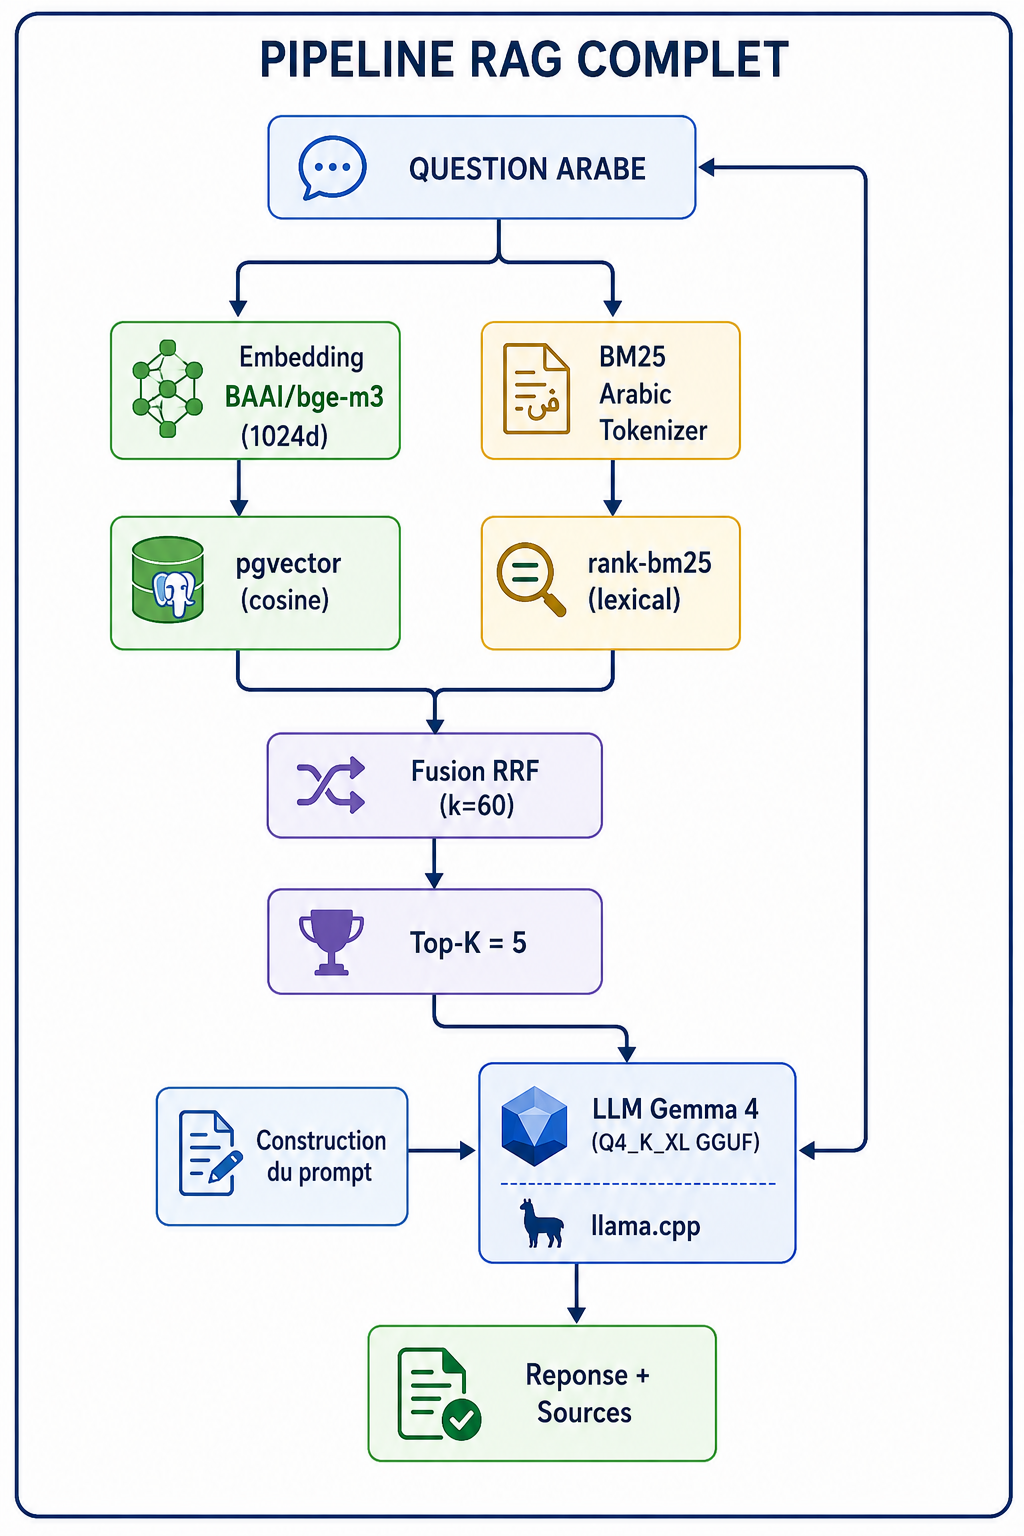
\includegraphics[width=0.6\textwidth]{images/illustrations/rag_pipeline_bge_m3.png}
    \caption{Complete hybrid Retrieval-Augmented Generation (RAG) pipeline for Arabic question answering.}
    \label{fig:hybrid-rag-pipeline}
\end{figure}


Cette approche garantit que chaque reponse est \textbf{tracable et verifiable} : l'utilisateur peut consulter les articles originaux ayant servi a la generation, et l'enrichissement contextuel (synthese, verdicts, references croisees) est explicitement distingue des hallucinations car ancre dans les sources.

\section{Technologies Utilisees}

Le systeme repose sur une stack technologique moderne et open-source, optimisee pour le deploiement sur materiel modeste :

\begin{itemize}
    \item \textbf{Extraction de texte} : PyMuPDF, pdfplumber, EasyOCR (reconnaissance arabe)
    \item \textbf{Correction OCR} : Modele de vision (VLM) Gemma 4 pour correction des erreurs de reconnaissance
    \item \textbf{Traitement du langage arabe} : Normalisation Unicode (NFKC), unification des alefs, suppression des tatweel, segmentation en articles, tokenizer arabe avec 60+ stop words juridiques
    \item \textbf{Modeles d'embedding} : intfloat/multilingual-E5-large (1024 dimensions, 560M parametres), BGE-M3 en alternative
    \item \textbf{Base de donnees vectorielle} : PostgreSQL 16 + pgvector 0.7.4 (indexation HNSW, m=16, ef\_construction=200)
    \item \textbf{Recherche hybride} : Similarite cosinus vectorielle + BM25 avec tokenizer arabe, fusion par Reciprocal Rank Fusion (RRF, k=60)
    \item \textbf{Modele de langage} : Gemma 4 2B parametres, quantifie Q4\_K\_XL (GGUF, $\sim$1.1 Go), inference via llama.cpp
    \item \textbf{Service d'embedding distant} : Google Colab (GPU T4) + Cloudflare Tunnel pour l'embedding GPU, fallback CPU local
    \item \textbf{API Backend} : FastAPI (Python), endpoints REST (/search, /ask, /laws, /upload)
    \item \textbf{Frontend} : SvelteKit 5 + Tailwind CSS 4 + TypeScript
    \item \textbf{Infrastructure} : Docker Compose (PostgreSQL + pgAdmin), Cloudflare Tunnel, llama.cpp
\end{itemize}

\section{Domaines Juridiques Couverts}

Le systeme couvre sept domaines du droit marocain, avec un corpus d'environ 2 357 articles structures :

\begin{multicols}{2}
\begin{itemize}
    \item Droit Penal --- \textit{\textarabic{القانون الجنائي}} (822 articles)
    \item Code de la Route --- \textit{\textarabic{مدونة السير}} (228 articles)
    \item Droit Civil --- \textit{\textarabic{قانون الالتزامات والعقود}} (705 articles)
    \item Droit Commercial --- \textit{\textarabic{مدونة التجارة}} (359 articles)
    \item Procedures Judiciaires --- \textit{\textarabic{التنظيم القضائي}} (32 articles)
    \item Droit Fiscal --- \textit{\textarabic{المدونة العامة للضرائب}} (211 articles)
    \item Contraventions et Sanctions --- \textit{\textarabic{قانون المخالفات والعقوبات}}
\end{itemize}
\end{multicols}
